%%%% Better Poster latex template example v1.0 (2019/04/04)
%%%% GNU General Public License v3.0
%%%% Rafael Bailo
%%%% https://github.com/rafaelbailo/betterposter-latex-template
%%%% 
%%%% Original design from Mike Morrison
%%%% https://twitter.com/mikemorrison

\documentclass[a0paper,fleqn]{betterposter}

\usepackage[backend=biber,style=ieee,doi=false,isbn=false,url=false]{biblatex} %added
\addbibresource{refs.bib} %added
\renewcommand*{\bibfont}{\Large}
\usepackage{physics}
\usepackage{minted}
%%%% Uncomment the following commands to customise the format

%% Setting the width of columns
% Left column
\setlength{\leftbarwidth}{0.35\paperwidth}
% Right column
\setlength{\rightbarwidth}{0.25\paperwidth}

%% Setting the column margins
% Horizontal margin
%\setlength{\columnmarginvertical}{0.05\paperheight}
% Vertical margin
%\setlength{\columnmarginhorizontal}{0.05\paperheight}
% Horizontal margin for the main column
%\setlength{\maincolumnmarginvertical}{0.15\paperheight}
% Vertical margin for the main column
%\setlength{\maincolumnmarginhorizontal}{0.15\paperheight}

%% Changing font sizes
% Text font
%\renewcommand{\fontsizestandard}{\fontsize{28}{35} \selectfont}
% Main column font
%\renewcommand{\fontsizemain}{\fontsize{28}{35} \selectfont}
% Title font
%\renewcommand{\fontsizetitle}{\fontsize{28}{35} \selectfont}
% Author font
%\renewcommand{\fontsizeauthor}{\fontsize{28}{35} \selectfont}
% Section font
%\renewcommand{\fontsizesection}{\fontsize{28}{35} \selectfont}

%% Changing font sizes for a specific text segment
% Place the text inside brackets:
% {\fontsize{28}{35} \selectfont Your text goes here}

%% Changing colours
% Background of side columns
%\renewcommand{\columnbackgroundcolor}{black}
% Font of side columns
%\renewcommand{\columnfontcolor}{gray}
% Background of main column
%\renewcommand{\maincolumnbackgroundcolor}{empirical}
%\renewcommand{\maincolumnbackgroundcolor}{theory}
%\renewcommand{\maincolumnbackgroundcolor}{methods}
%\renewcommand{\maincolumnbackgroundcolor}{intervention}
% Font of main column
%\renewcommand{\maincolumnfontcolor}{gray}

\begin{document}	
\betterposter{
%%%%%%%% MAIN COLUMN

\maincolumn{
%%%% Main space

The appropriate \textbf{level of abstraction} for computational chemistry workflows is that of a \textbf{domain specific programming language} (DSL).
\vspace{2em}

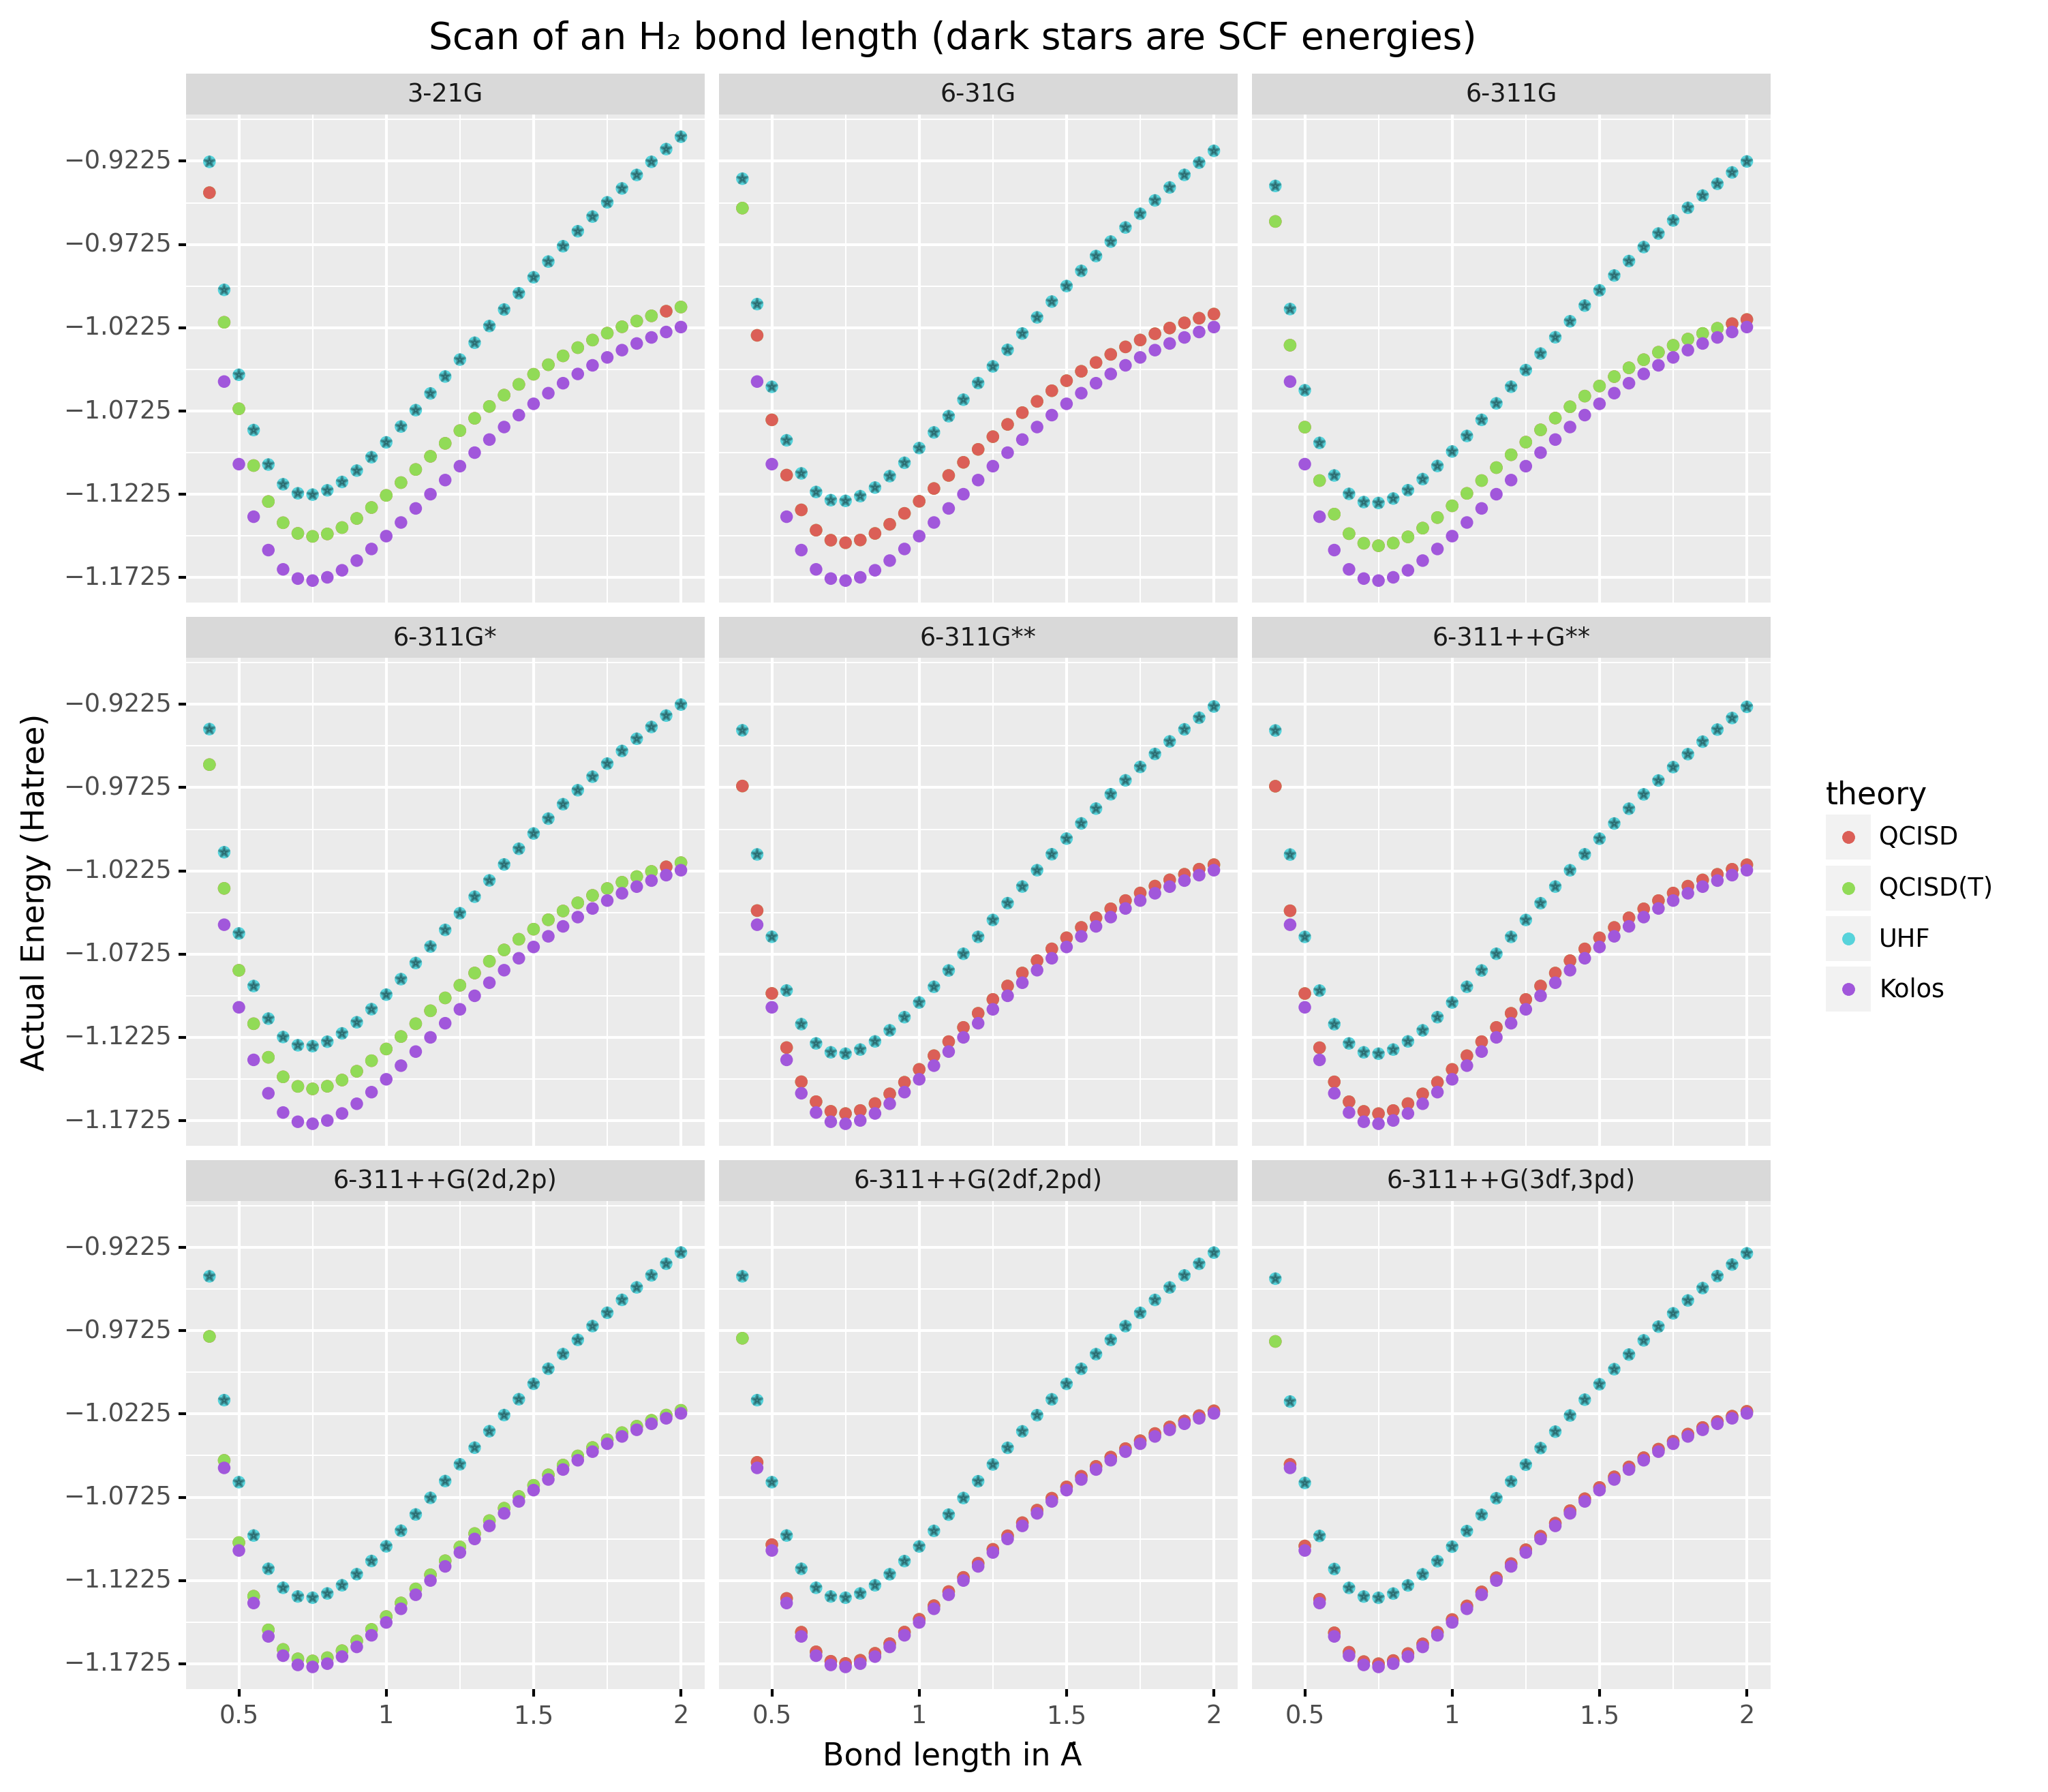
\includegraphics[width=\textwidth]{img/plotH2A.png}

{\fontsizetitle \textbf{$\dag$}} Data --> \texttt{parsimonious}
\vspace{1em}\\
{\fontsizetitle \textbf{$\dag$}} Outputs --> \texttt{pandas} data-frames
\vspace{1em}\\
{\fontsizetitle \textbf{$\dag$}} Units --> \texttt{pint}
\vspace{1em}\\
{\fontsizetitle \textbf{$\dag$}} Experiments defined as \texttt{cookiecutter} templates with metadata
\vspace{1em}\\
{\fontsizetitle \textbf{$\dag$}} Reliable output structured without user intervention
\vspace{1em}\\

}{
%%%% Bottom space

\vspace{1em}
%% QR code
\qrcode{img/SciPyConProceedingsWailordReview}{img/smartphoneWhite}{
\textbf{Take a picture} to
\\download the full paper
}
% Smartphone icon
% Author: Freepik
% Retrieved from: https://www.flaticon.com/free-icon/smartphone_65680

%% Compact QR code (comment the previous command and uncomment this one to switch)
%\compactqrcode{img/qrcode}{
%\textbf{Take a picture} to
%\\download the full paper
%}
\vspace{1em}
\fontsizestandard
Partially supported by the \textbf{Icelandic Research Fund}, grant number 217436052.

}

}{
%%%%%%%% LEFT COLUMN

\title{Wailord: Parsers and Reproducibility for Quantum Chemistry}
\author{Rohit Goswami$^{*}$}
\institution{Science Institute, University of Iceland}
\institution{Quansight Austin, TX, USA}
\institution{$^{*}$rog32@hi.is}

\section{Introduction}
Computers are meant to provide insights, not numbers. To this end however, the
ability to phrase chemical questions in a manner best suited to the efficient
and reproducible workflows is of paramount importance.

\section{Design Principles}

Data generation involves set of known configurations (say, \texttt{xyz} inputs) and a
series of common calculations whose outputs are required. Computational
chemistry packages tend to be focused on acceleration and setup details on a
\textit{per-job} scale. \texttt{wailord}, in contrast, considers the outputs of simulations
to form a tree, where the actual run and its inputs are the leaves, and each
layer of the tree structure holds information which is collated into a single
dataframe which is presented to the user.

\texttt{wailord} leverages tools and methodologies from programming language
design leading to a robust and modular tool-chain.

ORCA (version 4) forms the computational core of the package.

Each segment is unit-tested to ensure reproducible results, and the design is modular enough to be expanded into more general purpose usage as well.

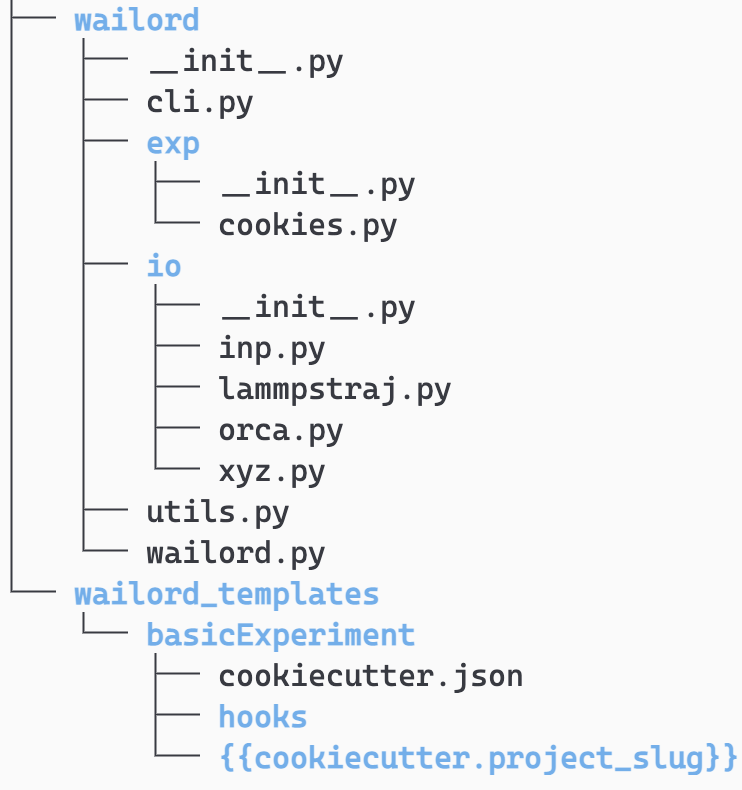
\includegraphics[width=0.8\textwidth]{img/wailordTreeStruct.png}


%% This fills the space between the content and the logo
\vfill

%% Institution logo

\includegraphics[width=0.5\textwidth]{img/affilUIRannisQS.png}

\includegraphics[width=0.5\textwidth]{img/scipyLogo22.png}\\

}{
%%%%%%%% RIGHT COLUMN

\section{Parsing Structures}
A grammar can be expressed as a series of tokens (terminal symbols) and
non-terminal (syntactic variables) symbols along with rules defining valid
combinations of these.

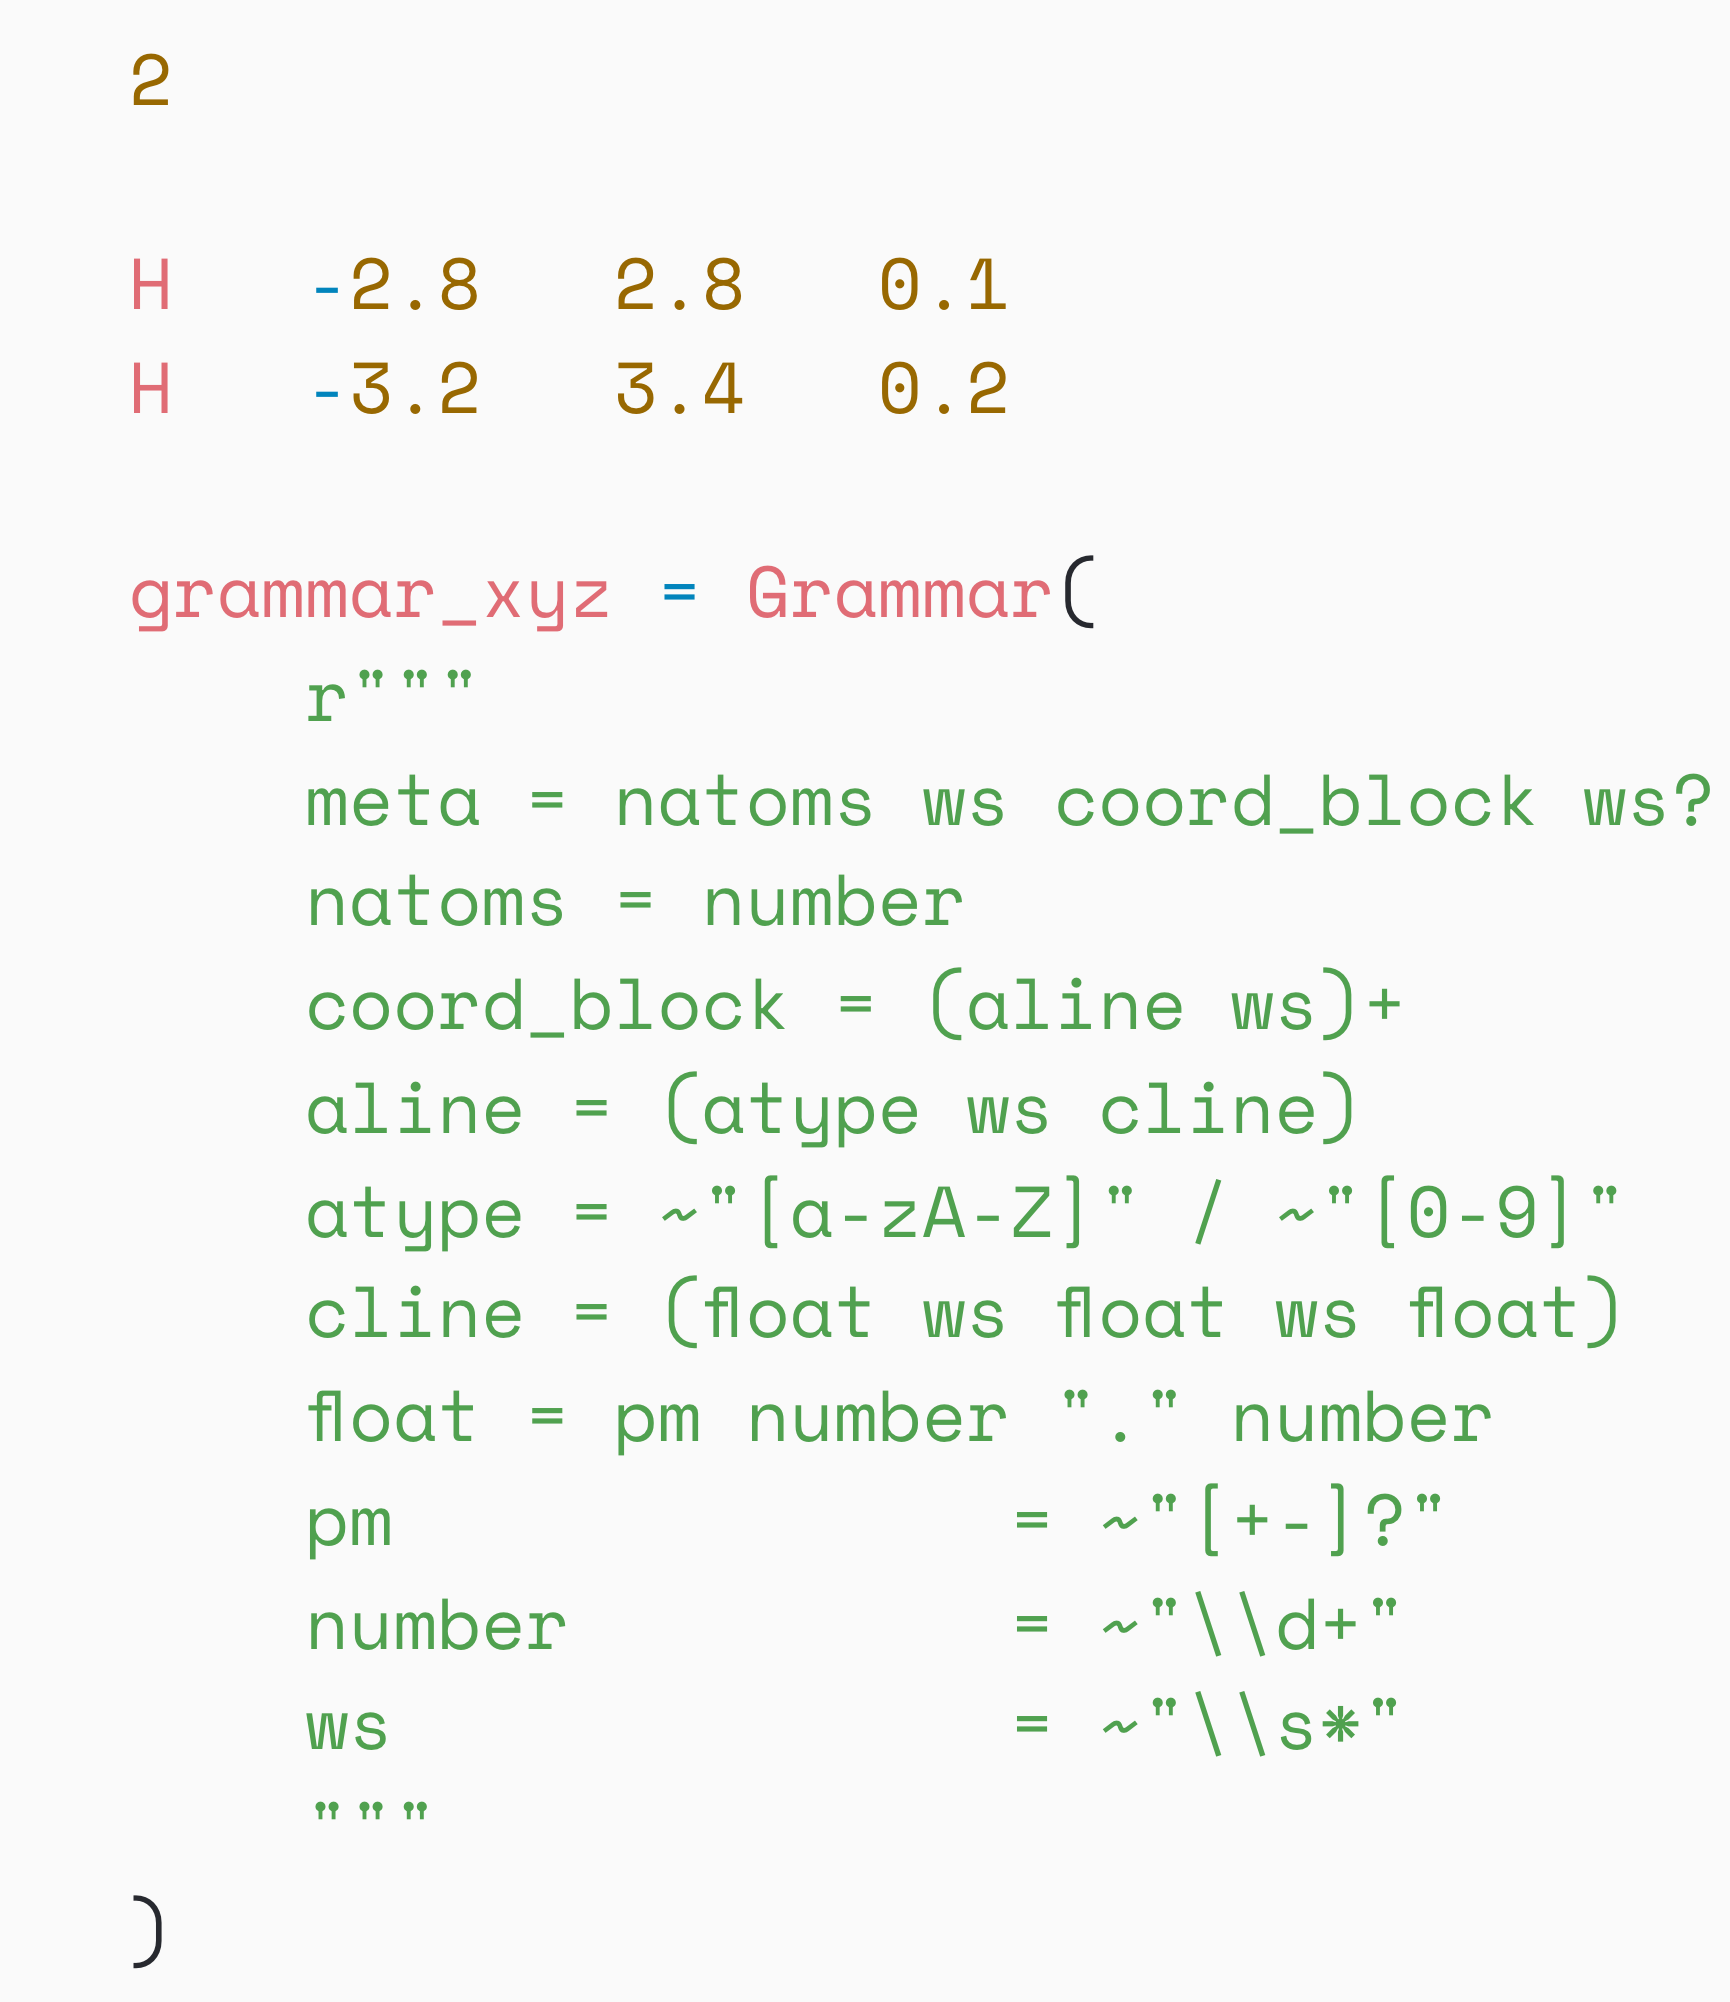
\includegraphics[width=\textwidth]{img/grammar_xyz.png}
\section{Generating Inputs}
Each "experiment" consists of multiple
single-shot runs; each of which can take a long time. A top level experiment is defined as:

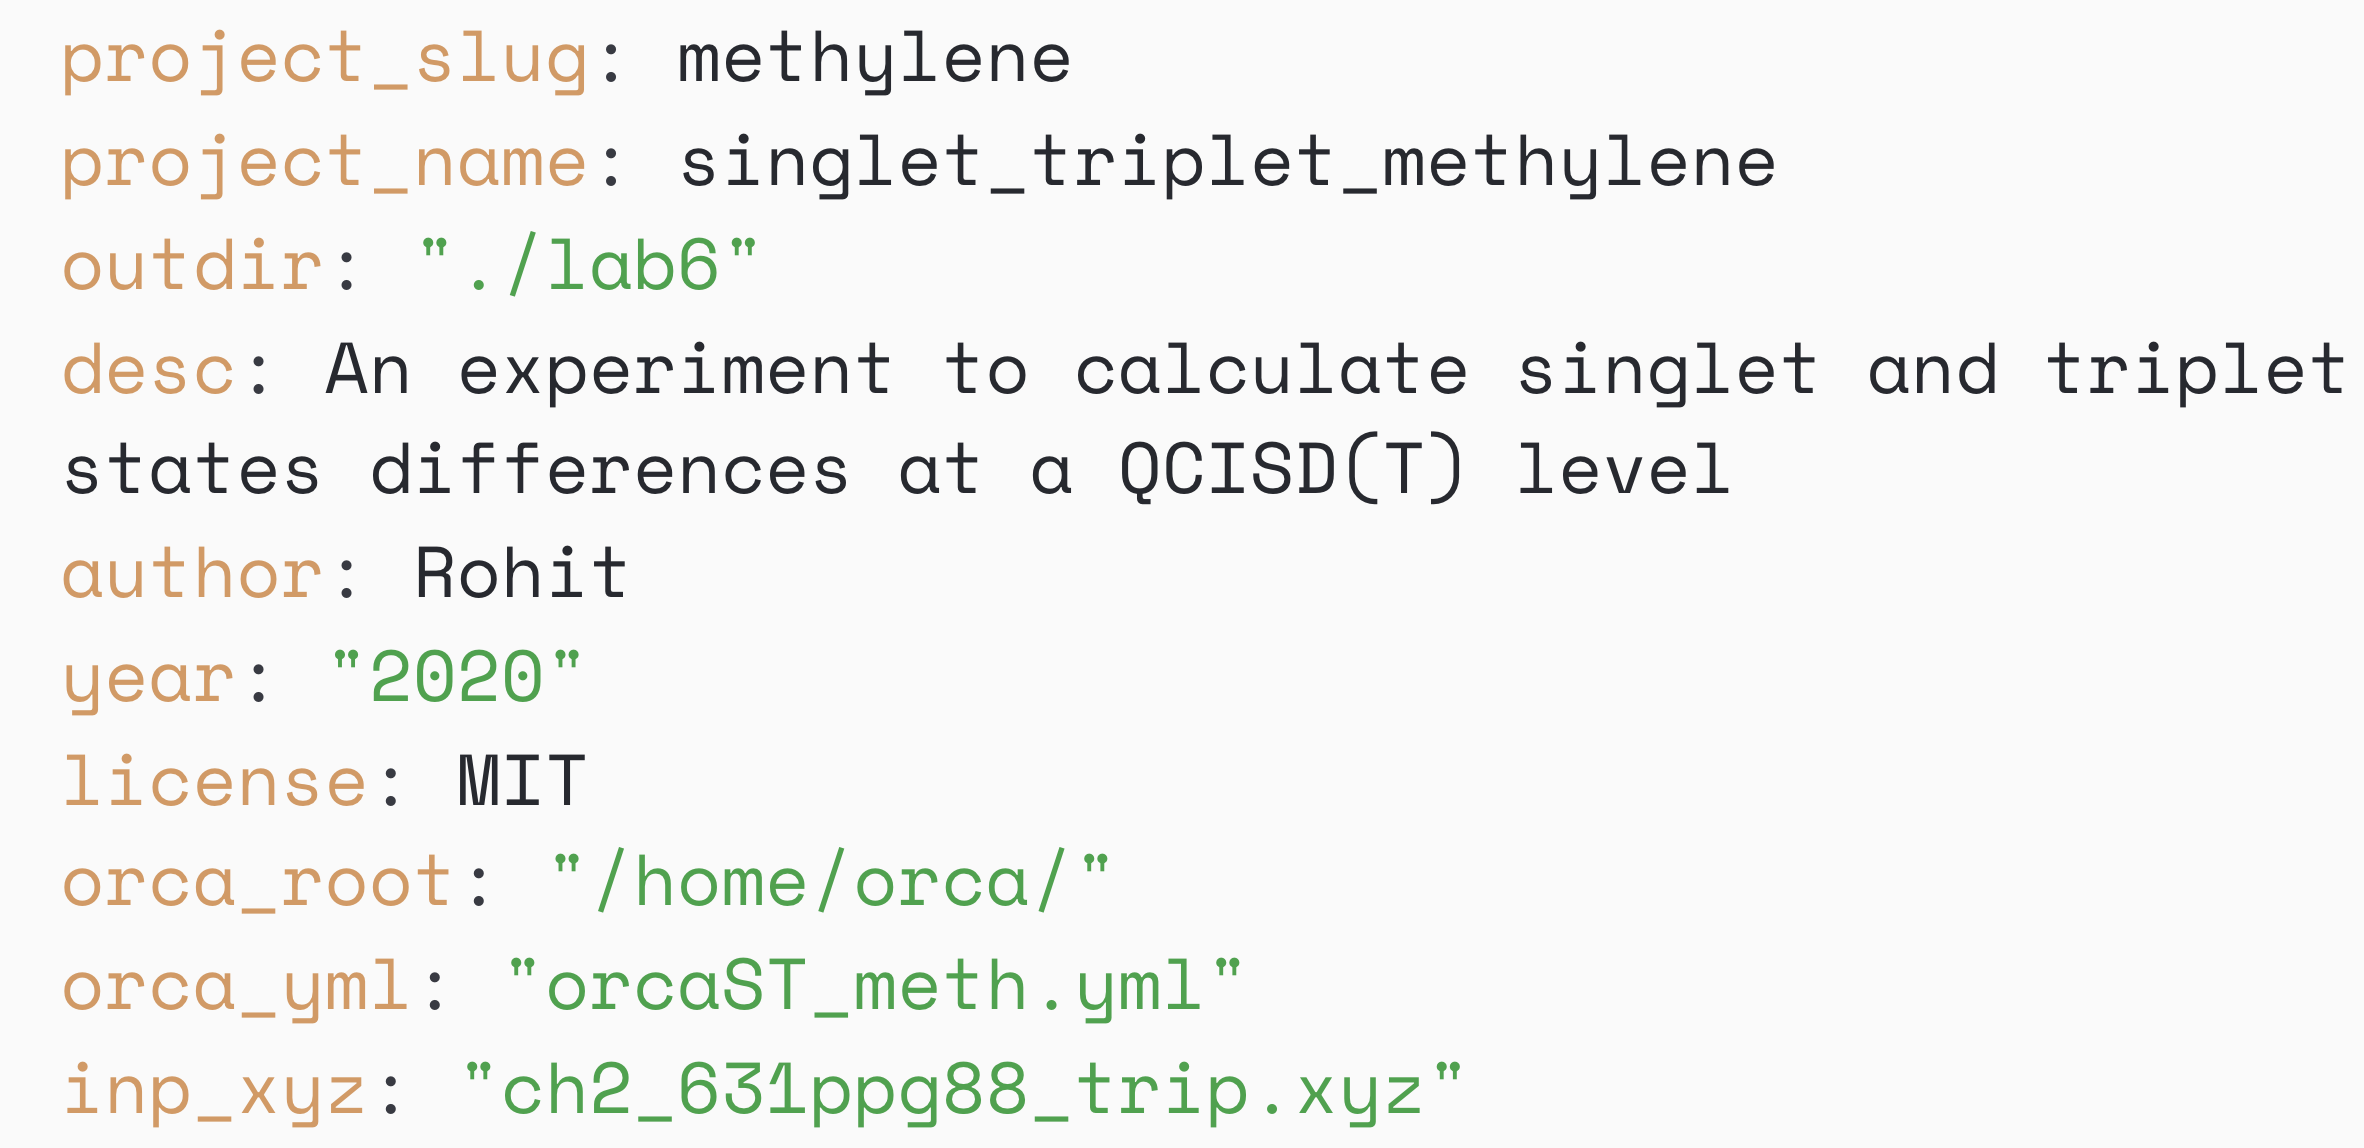
\includegraphics[width=\textwidth]{img/exampleExp.png}

Where each run is controlled individually.

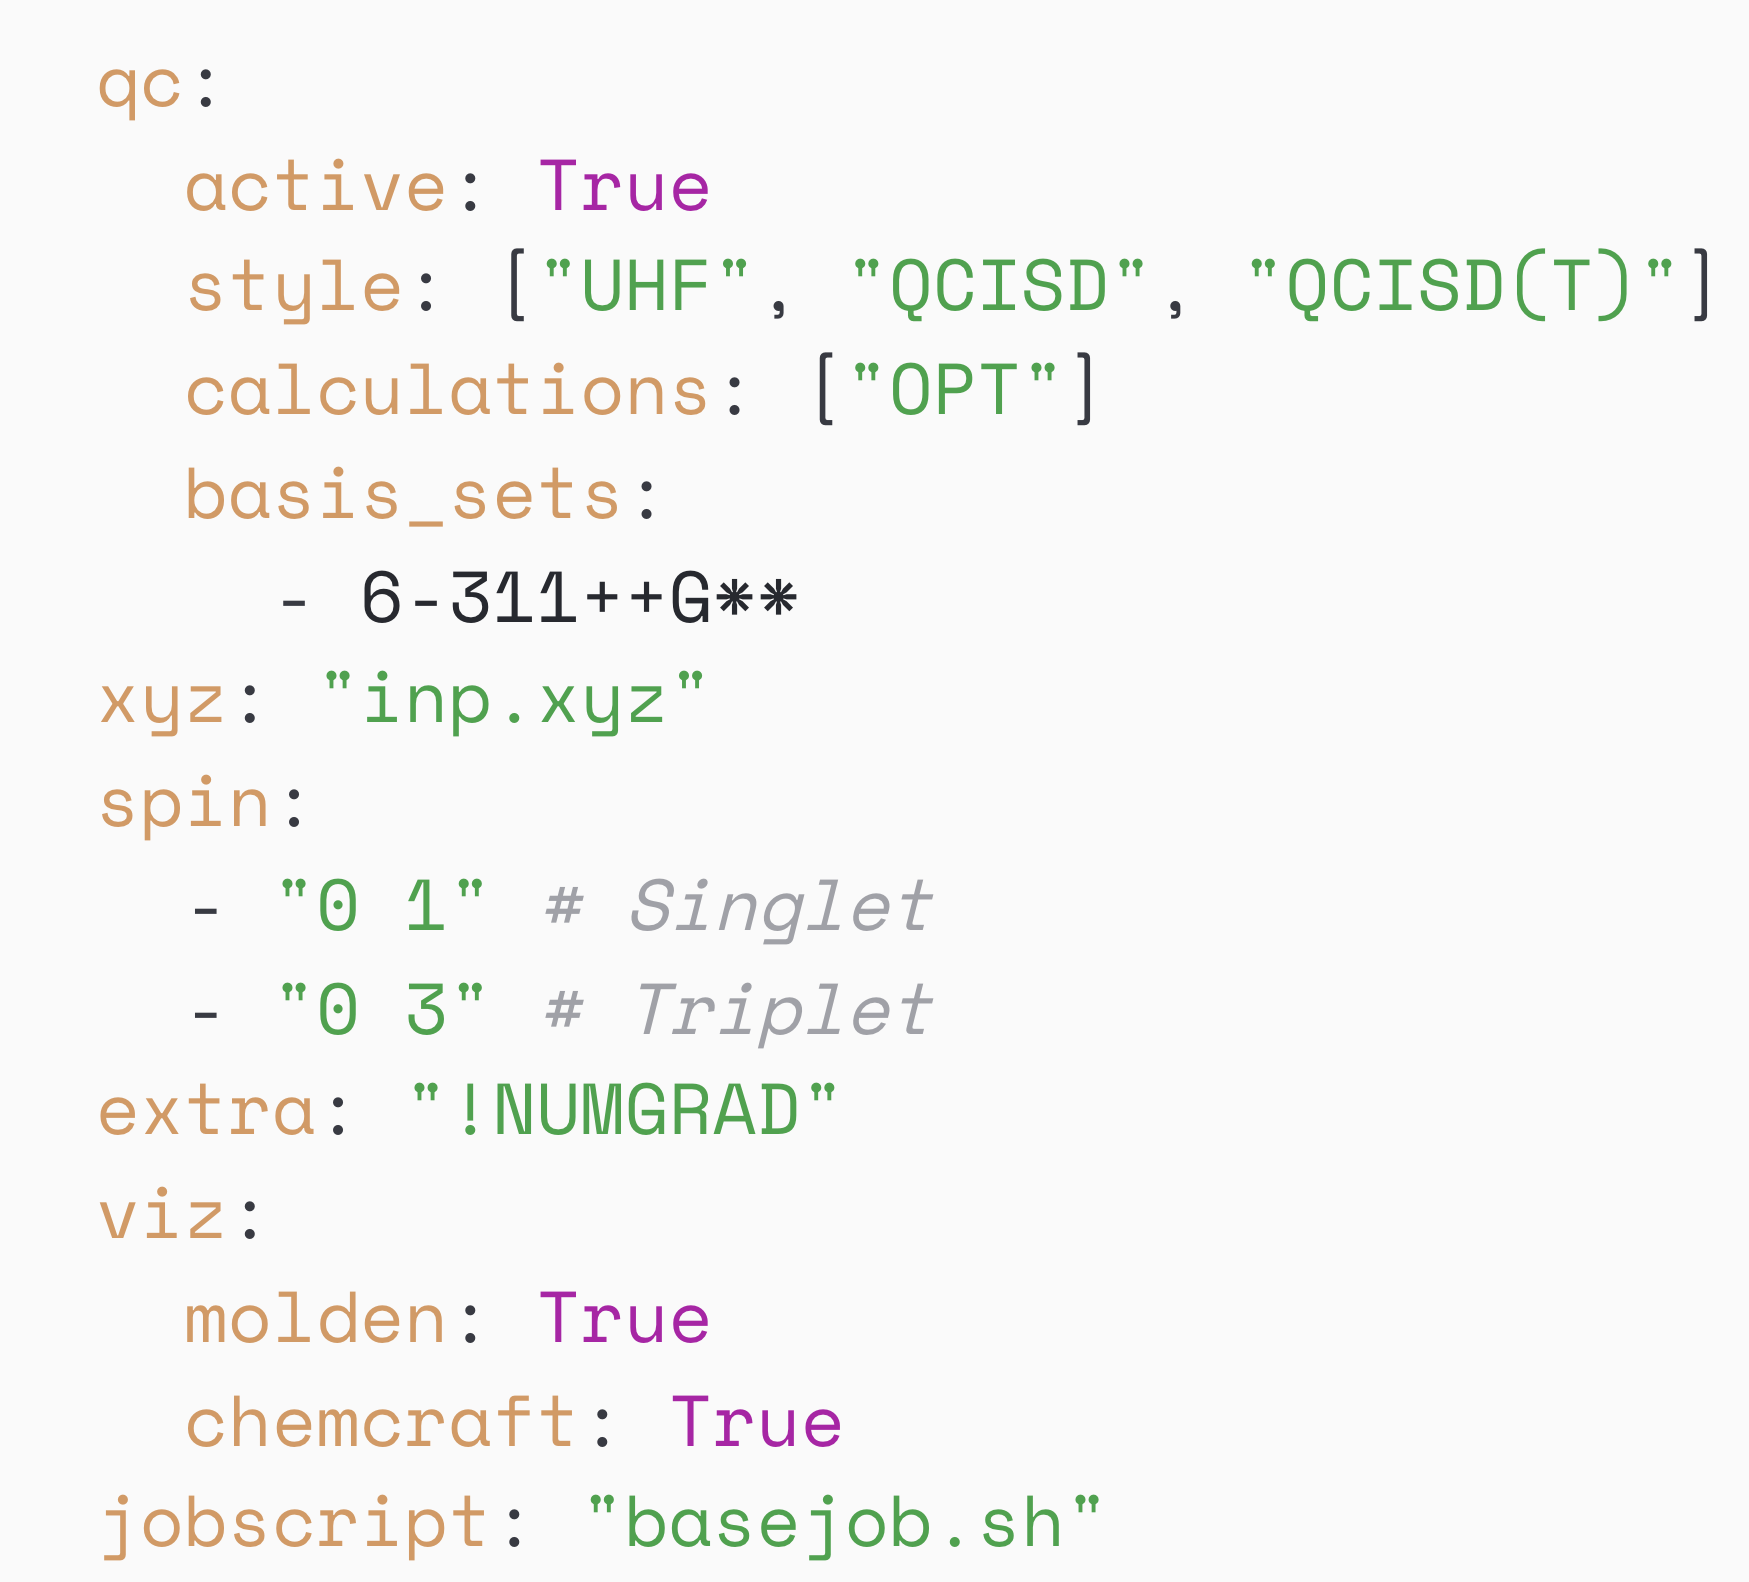
\includegraphics[width=\textwidth]{img/exampleRun.png}

With a directory tree generated by:

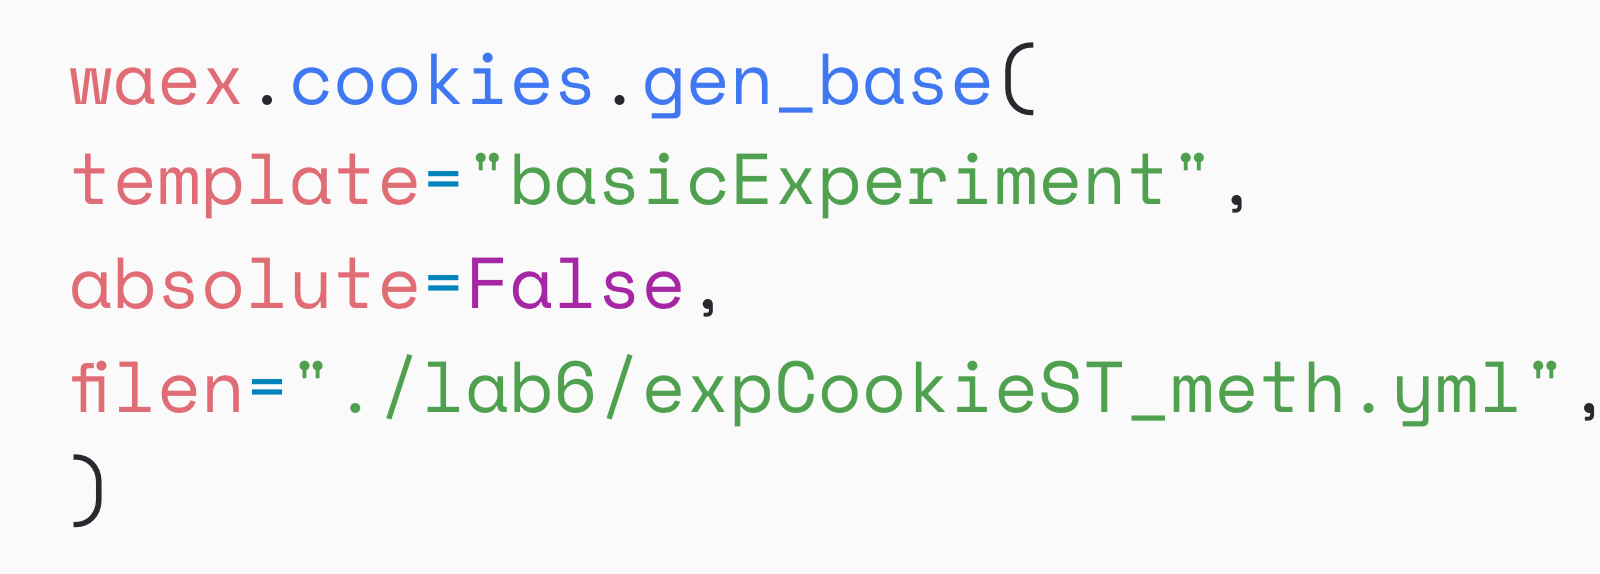
\includegraphics[width=\textwidth]{img/genDirTree.png}

Finally \texttt{pandas} data frames can be extracted from the outputs and analysis may be carried out say, in a \texttt{jupyter} notebook.

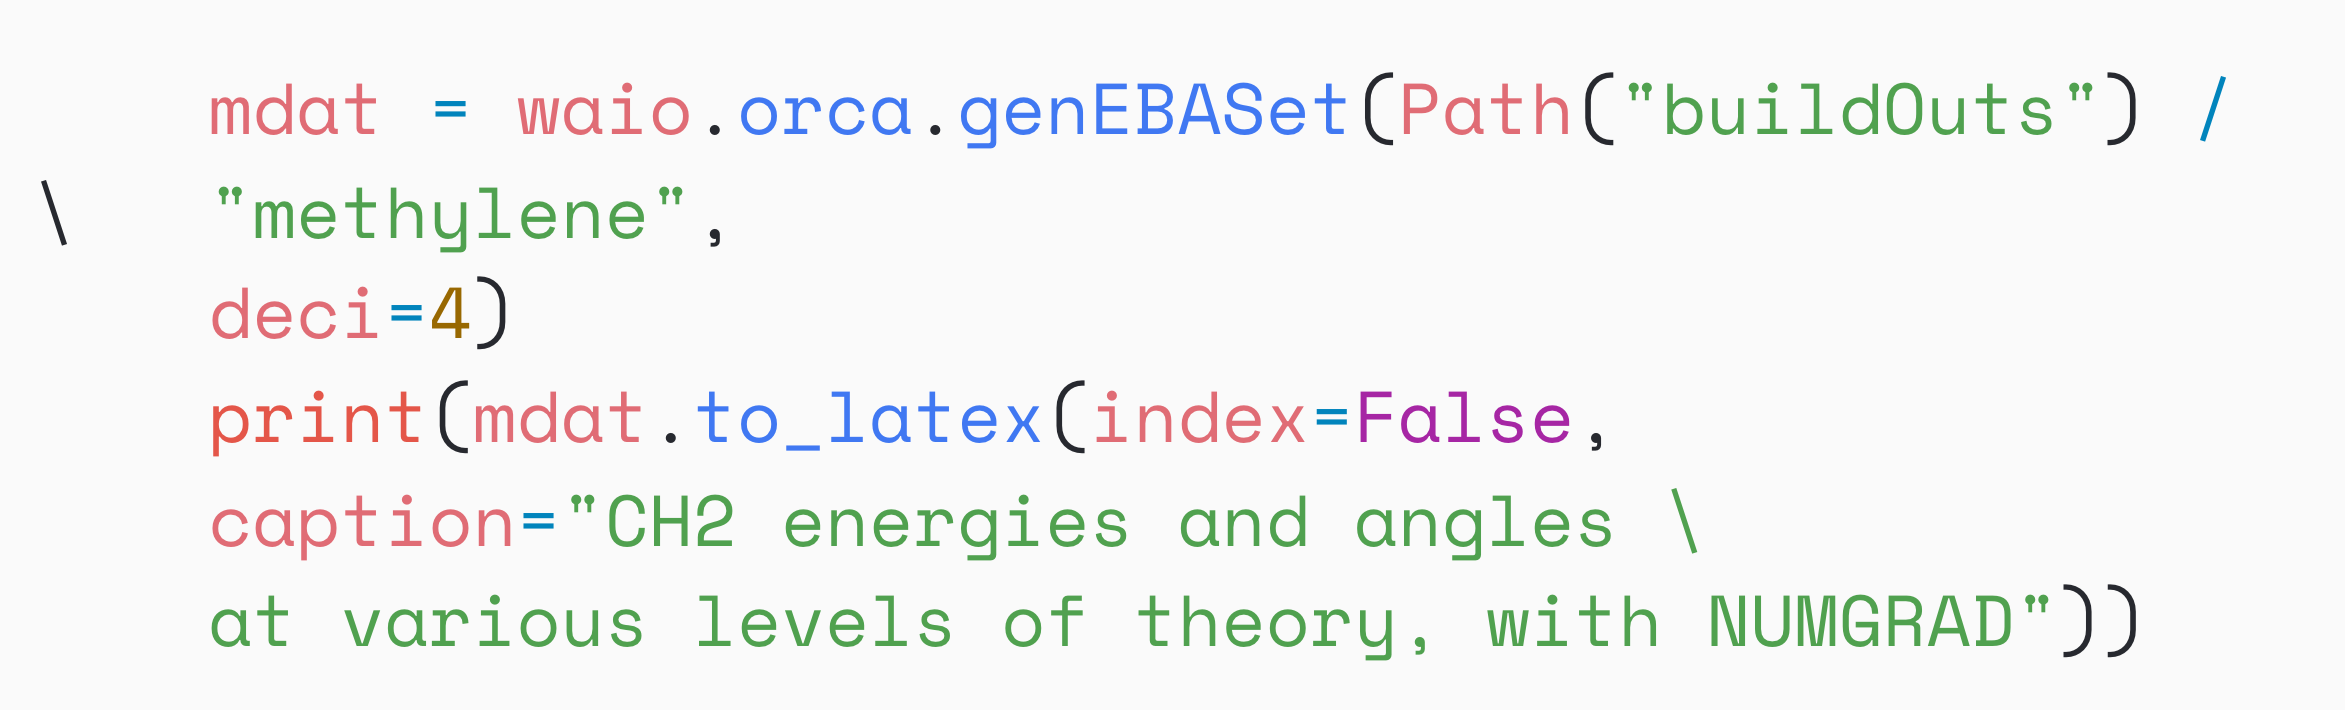
\includegraphics[width=\textwidth]{img/genEBA.png}

\section{References}
\nocite{ahoCompilersPrinciplesTechniques2007,sandveTenSimpleRules2013,pengReproducibleResearchComputational2011,oboyleCclibLibraryPackageindependent2008a,neeseORCAQuantumChemistry2020,kolosImprovedTheoreticalGround1968}
\printbibliography[heading=none] %added
}
\end{document}
